
%(BEGIN_QUESTION)
% Copyright 2007, Tony R. Kuphaldt, released under the Creative Commons Attribution License (v 1.0)
% This means you may do almost anything with this work of mine, so long as you give me proper credit

Digitale innganger på en PLS bruker ofte AC strømforsyning. AC inngangskretsen består som regel av en optokobler sammen med en likeretter med en stor motstand som største delen av spenningen skal legge seg over. Forklar hvordan denne kretsen virker. 

%Discrete (on/off) I/O for PLCs often works on AC (alternating current) power.  AC input circuitry usually consists of an optocoupler (LED) with rectification and a large dropping resistor to allow 120 volt AC operation.  AC output circuitry usually consists of TRIACs.  Explain how both of these technologies work.

\vskip 10pt

DC DI-er på en PLS består generalt av en optokobler og led, mens DO-er som regel har en transistor. I de følgende skjemaene vises noen eksempler. Legg merke til forskjellene. 

$$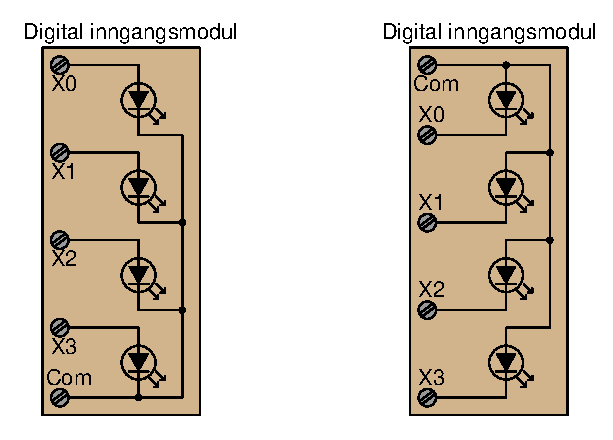
\includegraphics[width=15.5cm]{i02359x01.eps}$$

$$\includegraphics[width=15.5cm]{i02359x02.eps}$$

Finn ut om de ulike er inn- eller utganger og om de er \textit{sourcing} eller \textit{sinking}. 


\vskip 20pt \vbox{\hrule \hbox{\strut \vrule{} {\bf Suggestions for Socratic discussion} \vrule} \hrule}

\begin{itemize}
\item{} Determine how real input and output devices (e.g. switches, solenoid coils) would need to be connected to the I/O terminals of these modules.
\end{itemize}

\underbar{file i02359}
%(END_QUESTION)





%(BEGIN_ANSWER)


%(END_ANSWER)





%(BEGIN_NOTES)

Optocouplers use LEDs and phototransistors to couple discrete data from input to output optically, so there is no galvanic connection between input and output circuits.  This is useful in a PLC, so that the sensitive circuitry of a PLC's processor shares no electrical connections with the real-world inputs.

TRIACs are thyristor devices used to switch AC power.  Once triggered, they latch ``on'' until the current is externally halted, such as when current passes through 0 every half-cycle of an AC waveform.

\vskip 10pt

The key to understanding each designation is to draw an arrow for {\it conventional flow} at each I/O terminal (excluding the ``Common'' terminal).  An outward-pointing arrow (away from the module) represents sourcing I/O.  An inward-pointing arrow (toward the module) represents sinking I/O.

$$\includegraphics[width=15.5cm]{i02359x03.eps}$$

$$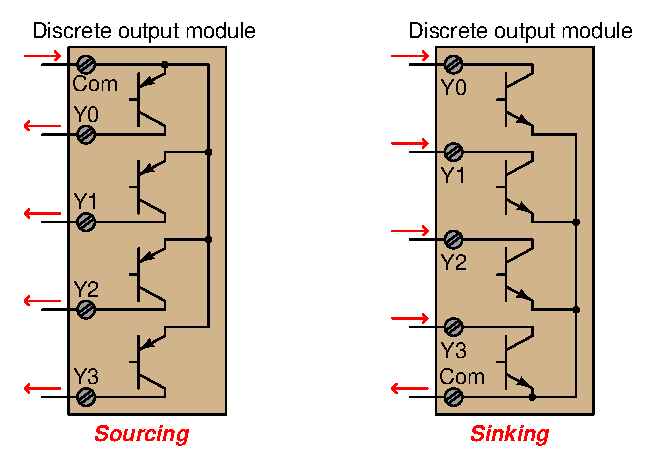
\includegraphics[width=15.5cm]{i02359x04.eps}$$

\vskip 10pt

A sourcing module needs to connect to a sinking device, and vice-versa.

%INDEX% PLC, I/O: sinking versus sourcing

%(END_NOTES)


